\documentclass[conference]{IEEEtran}
\usepackage{cite}
\usepackage{amsmath,amssymb,amsfonts}
\usepackage{algorithmic}
\usepackage{url}
\usepackage{graphicx}
\graphicspath{{./images/}}
\usepackage{textcomp}
\usepackage{xcolor}
\usepackage{listings}
\usepackage[utf8]{inputenc}
\usepackage[T1]{fontenc}
\usepackage{pgf}
\usepackage{pgf-umlsd}
\usepackage{pgf-umlcd}
\usepackage{tikz}
\usepackage{tikz-uml}
\usetikzlibrary{positioning,shapes.multipart}
\usepackage{pgf}
\usetikzlibrary{positioning}

\def\BibTeX{{\rm B\kern-.05em{\sc i\kern-.025em b}\kern-.08em
    T\kern-.1667em\lower.7ex\hbox{E}\kern-.125emX}}

% Preamble for page numbering

\pagestyle{plain}
\pagenumbering{arabic} % Other options: roman, Roman, alph, Alph

\begin{document}

\title{MorteSense \\DIY Home Security}

\author{\IEEEauthorblockN{Shohin Abdulkhamidov}
      \IEEEauthorblockA{\textit{Dept. of Computer Science} \\
            \textit{San Jose State University}\\
            San Jose, United States \\
            shohin.abdulkhamidov@sjsu.edu}
      \and
      \IEEEauthorblockN{Diego Cruz}
      \IEEEauthorblockA{\textit{Dept. of Computer Science} \\
            \textit{San Jose State University}\\
            San Jose, United States \\
            diego.cruz@sjsu.edu}
      \and
      \IEEEauthorblockN{Diego Garcia-Carrasco}
      \IEEEauthorblockA{\textit{Dept. of Computer Science} \\
            \textit{San Jose State University}\\
            San Jose, United States \\
            diego.garciacarrasco@sjsu.edu}
      \and
      \IEEEauthorblockN{Spartak Gevorgyan}
      \IEEEauthorblockA{\textit{Dept. of Computer Science} \\
            \textit{San Jose State University}\\
            San Jose, United States \\
            spartak.gevorgyan@sjsu.edu}
      \and
      \IEEEauthorblockN{Faramarz Mortezaie}
      \IEEEauthorblockA{\textit{Dept. of Engineering} \\
            \textit{San Jose State University}\\
            San Jose, United States \\
            faramarz.mortezaie@sjsu.edu}
}

\maketitle

\begin{abstract}
      In recent years, DIY security system technologies have been simplified and became
      more affordable for the general public. This coincided with the emergence of brands
      like Ring, Blink, Wyze, SimpliSafe, and Vivint, which specialized in smart home
      security. These brands offer a range of products, including front-door cameras,
      infrared motion sensors/detectors, and in-home cameras providing various views of
      the house.

      One notable drawback of these product ecosystems is their reliance on a mobile
      application and a smartphone capable of running it. If the application ceased to
      receive support or the company went out of business, the associated hardware might
      no longer function as intended, resulting in unnecessary e-waste and unsustainable
      security practices.

      The project addressed the dependency on a smartphone application by utilizing SMS
      text messaging within a modular motion detection security system. The system is part
      of an ecosystem that could be customized to meet the user's specific requirements
      and specifications. It was designed with sustainability in mind, capable of
      persisting even if manufacturer support became unavailable.
\end{abstract}

\begin{IEEEkeywords}
      DIY, Home Security, Microcontroller, Open-Source
\end{IEEEkeywords}

\section{Project Overview}

\subsection{Project Goals and Objectives}
The MorteSense DIY security system, more accurately described as the Microwave Motion
Security System with SMS Notifications, was a project intended to provide efficient
and reliable security for homes and businesses. The system uses microwave motion sensors
to detect movement within a certain range and sends an SMS notification to the owner's
phone in case of any suspicious activity.

To manage the development process efficiently, the team followed the Agile Scrum framework.
The user stories in this project involved creating the sensor unit, communication module,
and SMS notification system. The Project requirements included designing an intuitive user
interface, ensuring compatibility with different devices, and developing a robust and
secure system that is easy to install and operate.

\subsection{Problem and Motivation}

The MorteSense project aims to address the growing need for accessible, cost-effective,
and reliable security solutions for residential and commercial properties. Traditional
security systems often come with high installation and maintenance costs and complex
setups, making them unattainable or impractical for many people.

The motivation behind MorteSense was to create a DIY security system that leverages
microwave motion detection technology to provide an affordable, easy-to-install, and
efficient means of monitoring and securing properties. This project is important as
it can pave the way to make more advanced security systems accessible to a wider
audience, thus improving safety and security for individuals and businesses.

To ensure real-time alerts, the system incorporates SMS notifications, which enable
swift responses to potential security breaches. This approach effectively addresses
the need for a more convenient and user-friendly security solution.

\subsection{Project Application and Impact}

In today's society, advanced security systems have become crucial in ensuring public
health, safety, and welfare. With growing concerns regarding security, the need for
efficient and reliable security systems is more pressing than ever. The Microwave
Motion Security System with SMS Notifications has gained popularity in recent years
due to its many benefits in preventing harm and property damage. This system has
been designed with critical factors such as global, cultural, societal, environmental,
and economic considerations in mind, ensuring accessibility and effectiveness for a
wider range of users.

Public health, safety, and welfare are essential considerations for any security system.
The microwave motion security system with SMS notifications can detect and notify
homeowners of potential security risks, which is vital for public safety. The SMS
notification feature allows prompt action to be taken, reducing the risk of harm
and property damage. By reducing crime rates in a neighborhood, the security system
can also positively impact the safety and well-being of the community. In case of a
security breach, the system can notify emergency services which minimizes damage and
protects lives.

\subsection{Project Results and Deliverables}

\subsubsection{Project Results}

The project results include a microcontroller and microwave motion sensor enclosed inside of a 3D-printed case DIY motion detector, and a deployed User Management Services (UI) in Amazon AWS.

\subsubsection{Deliverables}

The following are the deliverables set during Spring 2023:
\begin{itemize}
      \item High-Level requirements
      \item Software Requirements Specification document
      \item Roadmap
            \subitem This involved a conversion of the provided schedule document from CMPE 195A into a Gantt Chart
      \item Software Backlog
            \subitem Involved documenting different product features and specifications according to the requirements, then assigning different people to implement them
      \item Hardware Backlog
            \subitem Involved documenting the history of making changes to the hardware, and figuring out the best implementations among the different configurations
            \subitem Will mostly fall under internal-use, but was occasionally referenced or drawn upon for project submissions
\end{itemize}

The following are the deliverables set during Summer 2023:
\begin{itemize}
      \item Creation of CAD Specification Document that will outline the
            constraints that the enclosure(s) must follow for the system
            \subitem Iterative revisions of the 3D-printed enclosure(s) will follow
            \subsubitem Likely will be logged in hardware backlog document
      \item A prototype enclosure for the central module is expected at the end of Summer 2023
\end{itemize}

The following are the deliverables set during Fall 2023:
\begin{itemize}
      \item Start of development
            \subitem Involved assembling the initial prototype of the hardware and coding
            the network communication between hardware and software
            \subitem Set up the communication of the microcontroller and motion detector
            \subitem The Backend API was initialized and deployed, Twilio gateway was pushed to Fall 2023
      \item Creation of a CAD Specification document that will outline the constraints
            that the enclosure(s) must follow for the system
            \subitem Iterative revisions of 3D-printed enclosure(s) were done throughout the
            semester
            \subitem Was logged in the hardware backlog and followed previously mentioned rules
      \item Integration with Amazon AWS
            \subitem Integration of the User Management Service (UI) into the backend
            \subitem Deployment and integration of Amazon AWS cloud computing,
            analytics, and reporting services.
      \item More Testing and Configuration
      \item Final Deliverables
            \subitem Hardware is enclosed in a 3D-printed case
            \subitem Final Project Presentation
\end{itemize}

\section{Background and related Work}

\subsection{Background and Technologies}

In recent years, DIY home security has risen in popularity, with modern solutions including
doorbell cameras, fingerprint-scanning door modules, infrared motion detection sensors, and
the occasional surveillance camera. Companies like Ring, Blink, Wyze, SimpliSafe, and Vivint
have had a significant impact on improving the availability of home security and in the
development of smart homes that are connected to the Internet of Things (IoT).

Leading up to this point, contemporary literature has explored how using different parts
from different manufacturers in unique configurations can be integrated into
IoT \cite{sarhan2020}. Additionally, current literature explores how DIY home security
will develop in relation to the blockchain \cite{arifEtAl_2020} and the growing influence
of machine learning\cite{khanEtAl2021}.

In light of this related work, this project entailed creating a DIY security system that
will utilize contemporary microcontrollers and microwave motion detection sensors and
will be able to interface with mini-motion proximity cameras. Modular design principles
were used to create an efficient, small-scale security system that can add different access
points through different modules. Combined with extensive documentation, users are able
to test, maintain, and repair the system as needed.

In addition to using modular design principles, modern technologies including using Wi-Fi
to connect to remote servers and notify users of events with SMS text messaging as well
as web protocols to broadcast the history of detections/captures and enact security
network management, allow for an open ecosystem that can be tailored to the user’s
requirements/specifications and remain sustainable by persisting even if direct
manufacturer support is no longer available.

In the context of this project, the DIY security system builds upon the work established
by research conducted by IEEE engineers and scientists that used the Arduino and
Raspberry Pi platform. This project explored cutting-edge devices and technologies
that were not necessarily present at the time of previous studies, and further analysis
is given in the State of the Art section following this literature review.

Komninos et al. explores the threats to smart homes and smart grids with respect to
software security and attacks involving invasions. This study uncovered that smart grids
have the threat of message modifications, replay attacks, metric impersonation, and
denial-of-service, while smart homes have similar threats, with unique ones including
false synchronization and eavesdropping \cite{komninosEtAl2014}. The main concerns for
current smart homes now include false synchronization and denial-of-service, being the
most convenient methods for burglars to effectively invade and loot a home. The two
aforementioned attacks were taken into account when developing the DIY security system,
learning from the limitations of this particular study.

A 2017 study conducted by two IEEE researchers explored the vulnerabilities that existed
in DIY home security systems that used sensors, microcontrollers, Raspberry Pi, and ZigBee
communications \cite{joseMalekian2017}. Jose and Malekian found that one limitation of
these systems at the time included the lack of an algorithm used to understand typical
user behavior and tripping an alarm when the algorithm judges the detected behavior as
erratic. Another limitation of systems at the time was that the ZigBee and IEEE 802.15.4
communications protocol were susceptible to replay attacks, allowing attackers familiar
with the technology to exploit the vulnerability and intrude
into the home \cite{joseMalekian2017}.

Arif et al. examined the development of blockchain technology and its ability to
handle great demand in its use cases. They evaluated the possibility of using blockchain
technology to back IoT devices in DIY smart home security with a proposed blockchain
configuration (see Appendix D). They found that while it was cost-effective and remained
independent of cloud storage, the computation difficulty was set to the lowest possible,
which may become complicated as more devices are added to the security system [4].
Variable computation difficulty is a new technique gaining popularity, but further
research was made on the hardware requirements, and it was found to require more
resources than what had been planned for the scope of the project.
This is because the project will include web services and a deliberately
designed user experience.

IEEE member Qusay Sarhan conducted a comprehensive literature review in 2020, providing an
overview of dozens of research reports on smart home safety and security systems that
used the Arduino platform. It was found that the most significant challenges to building
these systems included physical attacks, device failure (of microcontroller/module),
power/internet outages, and software compatibility \cite{sarhan2020}. These are factors
that weighed heavily on this project and provided a point of reference for further learning
and improving the work that has already been done in the field. Additionally, the review
provided a few subjects of interest, including extendability, performance, visualization,
and testing for stress/robustness \cite{sarhan2020}.

Lastly, Khan et al. built on the work conducted by Arif et al. by exploring the role that
machine learning could play in home security systems that utilize blockchain technology.
They found that using a Deep Extreme Learning Machine (DELM) combined with blockchain could
prove to be far more efficient compared to other algorithms \cite{khanEtAl2021}.
Using machine learning was beyond the scope of this project, but it is a valid
consideration in building upon the work for a graduate research project.

\subsection{State of the Art}

The current state-of-the-art home security systems employ different techniques and products
to create a comprehensive system that can typically be tailored to the end user through
the use of modules. These products are often well-established and are only revised in
ways that are not directly observable by the end user. Rather, the underlying technology
may change while the enclosure receives minor modifications at most \cite{sarhan2020}.
The most common implementation for state-of-the-art home security systems involves the
use of modules that connect wirelessly to a central unit through some wireless
protocol \cite{joseMalekian2017}. Alternatively, each individual module can connect
to the internet \cite{sarhan2020}. From there, the modules are handled by a mobile
application that allows the user to configure notifications for detection, remotely
set the alarm based on activity in the household, or remotely activate the alarm
from a safe place outside of the house if there is dangerous activity observed
within \cite{joseMalekian2017}.

Most modules are typically motion sensors or cameras, with motion sensors having had
much more development over the past few years compared to cameras. For the past
decade, motion sensors in DIY home security systems have used Passive Infrared (PIR)
technology to detect motion with changes in temperature induced by moving objects
compared to the ambient environment \cite{sarhan2020}. However, one limitation of
PIR sensors is that they cannot detect motion past objects, which means that large
furniture may prevent detection. Another limitation of PIR sensors is that their
perception of temperature may be thrown off by high ambient temperature or by wind,
meaning that if the weather is hot, it may not detect motion as a result of a
false negative, or if it is windy, it may create a false positive \cite{sarhan2020}.
In short, PIR sensors have a reduced effective distance because of the environmental
factors that can affect their ability to make accurate detections. Nonetheless, the
latest advancements have resulted in the recent acceptance of microwave motion
detector sensors that utilize the Doppler effect to detect motion behind objects
and are not susceptible to the environmental factors that impact PIR sensors \cite{sarhan2020}.
This means that cutting-edge DIY home security can more reliably detect motion behind
large furniture and can be installed outside of the house without as much concern for
environmental factors affecting the capacity to detect motion.

The Raspberry Pi and Arduino platforms have been extensively used as research tools
by the IEEE to explore different wireless communications technologies in the DIY
space, as well as for a central DIY security platform that is compared to established
home/personal security products \cite{sarhan2020}. Over the past decade, Arduinos and
their respective microcontrollers have increasingly used different connectivity types
such as XBee, Ethernet, and WiFi, most recently \cite{sarhan2020}. With the release of
the 802.11n-capable Raspberry Pi Pico W in 2022, the project builds upon the work
covered by previous research that used both mainline platforms or similar microcontrollers.

\section{Project Requirements}
\subsection{Domain and Business Requirements}
The MorteSense project had several requirements that the development team met to
create an efficient and reliable security system. These requirements included the
system's ability to detect motion accurately and differentiate between human and
non-human motion to avoid false alarms. Optional requirements included distinguishing
between different types of human motion, web-based monitoring and control, and a
built-in camera. The system's non-functional requirements included being reliable,
secure, easy to use, and having a long lifespan with minimal maintenance.

\subsection{System Functional Requirements}

Below are the functional requirements deemed essential for the project:
\begin{itemize}
      \item The system shall be able to detect motion accurately using microwave sensors with a range of at least 10 meters
      \item The system shall be able to send SMS notifications to a specific mobile device within 5 seconds of detecting motion
      \item The system shall have a built-in algorithm to differentiate between human motion and other types of motion, such as pets or moving objects, to avoid false alarms
      \item The system shall have a remote control that allows users to arm and disarm the system easily
      \item The system shall have a backup power supply that can provide at least 24 hours of continuous operation during power outages
\end{itemize}

The only functional requirement that was deemed desirable for the project involves the
system having a web-based interface that allows users to remotely monitor and control the
system, view motion event history, and adjust system settings.

\subsection{System Nonfunctional Requirements}

Below are the nonfunctional requirements deemed essential for this project:
\begin{itemize}
      \item The system shall be reliable and have a low false alarm rate of no more than 1%
      \item The system shall be easy to install and set up with clear instructions and user manuals provided
      \item The system shall be secure and prevent unapproved entery to private data or system configurations
\end{itemize}

Below are the nonfunctional requirements deemed desirable for this project:
\begin{itemize}
      \item The system should have a user-friendly interface that is intuitive and easy to use, with clear visual and auditory feedback provided
      \item The system should be design to have lower power consumption, consuming no more than 5 watts per hour to reduce operating costs
\end{itemize}

\subsection{Context and Interface Requirements}

With respect to interaction design, the team incorporated a user-friendly interface, clear
instructions, and collected feedback from the advisor and cohorts to ensure that the
security system was accessible to a broader audience, including older or less
technologically-savvy individuals, making it more effective and better-suited to the
intended audience.

\subsection{Technology and Resource Requirements}

There are several different resource requirements, and have been compiled into three
different categories: Hardware, Software, and Miscellaneous.

With respect to hardware, the resources used include a Raspberry Pi Pico W Microcontroller
with a 2.4GHz Wi-Fi Module furnishing, a 5.8GHz Microwave Motion Sensor, and the Thonny IDE
with Micropython. The Microcontroller is programmed to connect to the home Wi-Fi network and
send API requests to the backend server after processing motion detection data. The motion
sensor emits electromagnetic radiation that penetrates through non-solid objects and bounces
off solid objects. The Doppler effect is used to detect the slightest movement changes and
the sensor makes use of serial communications to exchange data between the microcontroller
and the motion sensor. This allows modification of sensitivity, distance, and other
parameters of the sensor. Thonny allows for compiling of Micropython into C code to
effectively program the hardware.

With respect to software, the resources used include the Python Flask framework for the
database server, ReactJS for the frontend, the Twilio API for notification service,
and Amazon AWS for cloud computing and reporting analysis. The Flask framework responds
to the provided hardware API requests and provides a web-based interace to allow users
to remotely monitor and control the system. The server functions as a gateway between
AWS services and a SQLite database to store and provide systems information. The
Twilio API is responsible for sending SMS notifications to client devices, and Amazon
AWS is responsible for handling and analyzing data traffic to provide different metrics
for what the sensor(s) report.

In terms of miscellaneous resource requirements, the Fritzing circuit design software,
SolidWorks CAD software, soldering tools, and 3D printing hardware were used to design,
simulate, and improve upon the hardware at different stages of assembly. Fritzing was
used during ideation to design and simulate the hardware scheme before actual assembly
and soldering. SolidWorks was used to design and prototype enclosures for the component
assembly, and was aided by the Makerspaces available at San Jose State University.

\section{System Design}

\subsection{Architecture Design}

\subsubsection{Project Hardware Architecture}

\begin{figure}[htbp]
      \centering
      \includegraphics[width=0.8\linewidth]{pcbDiagram.jpg}
      \caption{PCB Diagram}
      \label{fig:pcbDiagram}
\end{figure}

The PCB (Printed Circuit Board Diagram) diagram depicts the layout of the DIY security
circuit board. It shows the placement of components and their interconnections on the
board, as well as any necessary information related to the fabrication and assembly of
the board. While a circuit diagram provides a schematic representation of the electrical
connections between components, the PCB diagram shows the physical layout of the
components and the soldering points between them and the soldering layers. It is
important for the efficient routing of traces and connections and will be used during
the fabrication process.

The PCB will have 3 main components, the Raspberry Pi Pico W Microcontroller with
2.4Ghz Wi-Fi Module which is in the right top corner, the 9V Battery input in the
right bottom corner, and finally, it will have the 5.8Ghz Microwave Motion Sensor
which is in the left top corner of the board. The motion sensor emits electromagnetic
waves which are then reflected back to the receiver and analyzed. If the waves are
altered that means the object that reflected them is moving. The board also will have
4 LED indicators for showing the WI-FI connection indicator, power indicator,
motion detection indicator, and connection to backend service indicator.
Rx-Tx serial communication will be used between the microcontroller and motion sensor,
for all other communication GP pins will be used.

The hardware has two main components, the motion detector, and the microcontroller.
The microcontroller uses Rx-Tx serial communication to send and receive information
into the motion detector in the form of bits, which can be used to send and receive
instructions. Microwave Sensor out signal is used to detect the motion itself.
As the microcontroller comes with an integrated Wi-Fi module, it will be used to
communicate with the backend by sending and receiving API requests.
The device will enter sleep mode and only be activated during motion detection,
this will allow us to lower the power consumption significantly.
All the hardware will be programmed in C and Micropython.

The microcontroller has an integrated server with web UI, which allows users
to connect to it with their home devices such as smartphones, and do an easy setup
of the systems, such as the Wi-Fi module. UI also provides basic information regarding
the status of the motion detection device, battery lifetime, and other necessary
information. The microcontroller has full control over the motion detector which
allows users to do the precise configuration of system parameters, such as motion
detection range, sensitivity, etc.

\begin{figure}[htbp]
      \centering
      \includegraphics[width=1.5\linewidth, angle=-90]{hardwareArchitecture.jpg}
      \caption{Project Hardware Architecture}
      \label{fig:hardwareArchitecture}
\end{figure}

\subsubsection{Project Software Architecture}

The Notification Service is responsible for processing and sending SMS notifications
to users when the motion is detected. It receives the motion detection information
through requests from sensor management software and sends SMS notifications to the
registered mobile numbers. Notification Service will integrate SMS gateway using
Twilio API for communication with Client Devices. A database is required to store
information about the user systems, such as user information, sensor information,
and notification settings. The Reporting and Analytics component is responsible
for generating reports on the system’s performance, such as the number of motion
detections per day and average response time. It will help to analyze and further
improve the quality of the systems.


\begin{figure}
      \centering
      \begin{tikzpicture}[scale=0.65]
            \begin{umlcomponent}[x=4,y=0]{Cloud Workspace}
                  \umlbasiccomponent[x=1,y=-2]{User Management Service - UI}
                  \umlbasiccomponent[x=1,y=-4.5]{Reporting/Analytics Service}
                  \umlbasiccomponent[x=1,y=-6.8]{Database}
                  \begin{umlcomponent}[x=5.5,y=-3]{Notification Service}
                        \umlbasiccomponent[x=1, y=-2]{Twilio API}
                  \end{umlcomponent}
            \end{umlcomponent}
            \umlbasiccomponent[x=4.5,y=-10.6]{Sensor Management Software}
            \umlbasiccomponent[x=11,y=-10.6]{Client Device}

            % Bigger, thicker, and dashed arrows
            \draw[-latex, line width=1.5pt, dashed] (Sensor Management Software.north) -- (Notification Service.west);
            \draw[-latex, line width=1.5pt, dashed] (Twilio API.south) -- (Client Device.north);
      \end{tikzpicture}
      \caption{Software Architecture}
      \label{fig:softwareArchitecture}
\end{figure}



User Management Service (UI) will provide an interface for users to register and
authenticate their devices and configure notification settings. It will provide an
event log, which allows users to manage events related to sensors. Additionally, it
will have an audit trail of all activity in the system, including user activity.
The systems above will be powered by Amazon AWS, it allows us to expand and process
the volume of traffic.

\begin{figure}
      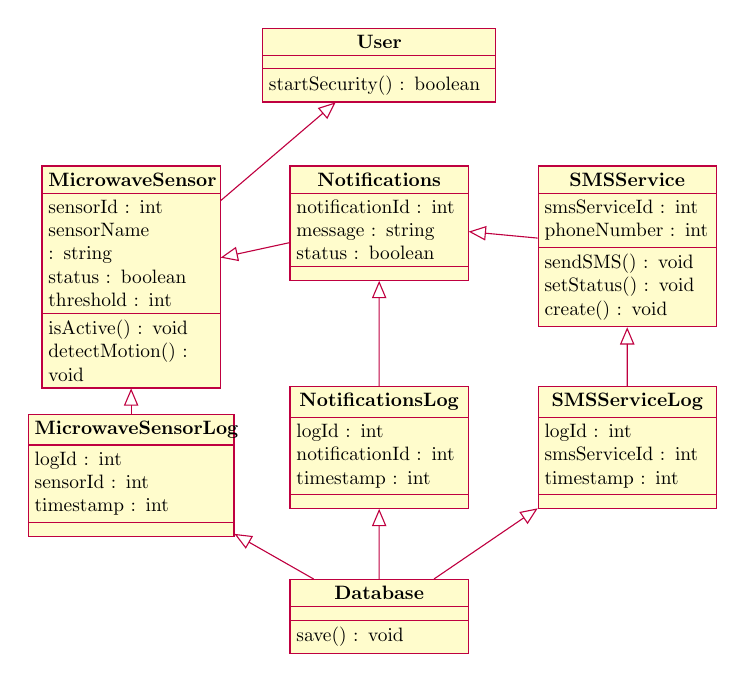
\begin{tikzpicture}[scale=0.7, every node/.style={scale=0.7}]

            \pgfdeclarelayer{background}
            \pgfdeclarelayer{foreground}
            \pgfdeclarelayer{connectionlayers}
            \pgfsetlayers{background,connectionlayers,main,foreground}

            \begin{class}[text width=4cm]{User}{4.5,0}
                  \operation{startSecurity() : boolean}
            \end{class}

            \begin{class}[text width=3cm]{MicrowaveSensor}{0 , -2.5}
                  \inherit{User}
                  \attribute{sensorId : int}
                  \attribute{sensorName : string}
                  \attribute{status : boolean}
                  \attribute{threshold : int}
                  \operation{isActive() : void}
                  \operation{detectMotion() : void}
            \end{class}

            \begin{class}[text width=3cm]{Notifications}{4.5 , -2.5}
                  \inherit{MicrowaveSensor}
                  \attribute{notificationId : int}
                  \attribute{message : string}
                  \attribute{status : boolean}
            \end{class}

            \begin{class}[text width=3cm]{SMSService}{9, -2.5}
                  \inherit{Notifications}
                  \attribute{smsServiceId : int}
                  \attribute{phoneNumber : int}
                  \operation{sendSMS() : void}
                  \operation{setStatus() : void}
                  \operation{create() : void}
            \end{class}
            \begin{class}[text width=3.5cm]{MicrowaveSensorLog}{0 , -7}
                  \inherit{MicrowaveSensor}
                  \attribute{logId : int}
                  \attribute{sensorId : int}
                  \attribute{timestamp : int}
            \end{class}

            \begin{class}[text width=3cm]{NotificationsLog}{4.5 , -6.5}
                  \inherit{Notifications}
                  \attribute{logId : int}
                  \attribute{notificationId : int}
                  \attribute{timestamp : int}
            \end{class}

            \begin{class}[text width=3cm]{SMSServiceLog}{9, -6.5}
                  \inherit{SMSService}
                  \attribute{logId : int}
                  \attribute{smsServiceId : int}
                  \attribute{timestamp : int}
            \end{class}

            \begin{class}[text width=3cm]{Database}{4.5 , -10}
                  \inherit{MicrowaveSensorLog}
                  \inherit{NotificationsLog}
                  \inherit{SMSServiceLog}
                  \operation{save() : void}
            \end{class}

      \end{tikzpicture}
      \caption{Software Class Diagram}
\end{figure}


The Class Diagram represents the relationships between various classes in the
Microwave Motion Security System with SMS Notifications. The User class is associated
with the MicrowaveSensor class, which is responsible for detecting motion.
The SMSService class is associated with the Database class, which is used to store
data related to the SMS services used to send SMS messages to the user.
The MicrowaveSensor class is associated with the Notification and SMSService classes,
which are responsible for sending notifications and SMS messages to the user when
motion is detected. These associations enable the MicrowaveSensor to trigger the
Notification and SMSService classes to send a notification and an SMS message
to the user, respectively.

The Database class is associated with the Notification, NotificationLog, SMSService,
SMSServiceLog, and SensorLog classes, which are used to store data related to
notifications, SMS services, and sensor logs. The Notification and SMSService
classes have a one-way association with the Database class, indicating that they
can use the Database to store data related to the notifications and SMS services
sent to the user. Additionally, the Notification and SMSService classes have
composition relationships with the NotificationLog and SMSServiceLog classes, respectively.
These composition relationships indicate that a Notification or a SMSService "has-a"
relationship with their respective log tables, and the log tables cannot exist
independently of the Notification or SMSService.

Finally, the SensorLog class has a one-way association with the MicrowaveSensor class,
which indicates that it can store data related to the logs of the microwave sensors
used for detecting motion. Overall, the Class Diagram demonstrates the flow of
information and data between the various classes and tables in the system, providing a
comprehensive representation of the Microwave Motion Security System with
SMS Notifications.


\begin{figure}
      \centering
      \begin{sequencediagram}
            \tikzstyle{inststyle}+=[bottom color=yellow]
            \tikzstyle{every node}+=[node distance=0.75cm and 0.75cm]

            \newthread{U}{:User}
            \newinst[0.75]{S}{:Sensor}
            \newinst[0.75]{T}{:Twilio}
            \newinst[0.75]{D}{:Database}

            \begin{sdblock}[green!20]{Device}{}
                  \begin{call}{U}{Create Device}{S}
                        {{\parbox{2cm}{\centering Acknowledge Device Creation}}}
                        \begin{call}{S}
                              {Store Device Data}{D}{Acknowledge Device Creation}
                        \end{call}
                  \end{call}
            \end{sdblock}

            \begin{sdblock}[green!20]{Connect Mobile}{}
                  \begin{call}{U}
                        {{\parbox{2cm}{\centering Connect to Phone}}}{S}
                        {{\parbox{2cm}{\centering Acknowledge Connection Update}}}
                        \begin{call}{S}{Update Connection Status}{D}{Ackn. Connection Update}
                        \end{call}
                  \end{call}
            \end{sdblock}

            \begin{sdblock}[green!20]{Subscribe to Alert}{}
                  \begin{call}{U}
                        {{\parbox{2cm}{\centering Subscribe to Alerts}}}{T}
                        {{\parbox{2cm}{\centering Provide User's Alert Preferences}}}
                        \begin{call}{T}
                              {{\parbox{2cm}{\centering Retrieve User's Alert Preferences}}}{D}
                              {{\parbox{3cm}{\centering Ackn. Subs.}}}
                        \end{call}
                  \end{call}
            \end{sdblock}

            \begin{sdblock}[green!20]{Receive Alert}{}
                  \begin{call}{U}{Request Alert}{S}{Notify User}
                        \begin{call}{S}{Retrieve Alert Data}{D}{Provide Alert Data}
                        \end{call}
                        \begin{call}{S}{Send Alert}{T}{}
                        \end{call}
                  \end{call}
            \end{sdblock}

      \end{sequencediagram}
      \caption{Software Sequence Diagram}
      \label{fig:softwareSeqDiagramUpdated}
\end{figure}

The sequence of events is as follows:
\begin{enumerate}
      \item The User triggers the Microwave Sensor to start monitoring for motion detection
            by calling the startSecurity() method.
      \item The MicrowaveSensor detects motion and triggers the Notification and SMSService
            to send a notification and an SMS message to the user, respectively.
      \item The Notification creates a new notification by calling the create() method,
            which generates a new notification ID.
      \item The Notification saves the notification data to the Database by calling the
            save(notification) method.
      \item The Notification sets the status of the notification to "sent" by calling the
            setStatus("sent") method.
      \item The SMSService creates a new SMS service by calling the create() method,
            which generates a new smsServiceId.
      \item The SMSService saves the SMS service data to the Database by calling the
            save(sms\_service) method.
      \item The SMSService sets the status of the SMS service to "sent" by calling the
            setStatus("sent") method.
      \item The SMSService sends an SMS message to the user by calling the sendSMS()
            method.
      \item The SMSService saves the log data related to the SMS message to the
            SMSServiceLog table by calling the save(sms\_service\_log) method.
      \item The Notification saves the log data related to the notification to the
            NotificationLog table by calling the save(notification\_log) method.
\end{enumerate}

In this way, the system can detect motion using the MicrowaveSensor, send notifications
and SMS messages to the user using the Notification and SMSService classes, respectively,
and store data related to these events using the Database, NotificationLog, and
SMSServiceLog tables.

\subsection{Design Constraints, Problems, Trade-offs, and Solutions}

\subsubsection{Design Constraints and Challenges}

Designing a DIY home security system presents several constraints and challenges that
require careful consideration. The primary requirement for the system is that it should
be easy to use, install, and work seamlessly across a diverse range of devices, which
necessitates careful consideration of the user interface and communication protocols.
Additionally, the system must be robust and secure to ensure that it is not easily
hacked or compromised. This requires implementing encryption and secure data storage
methods. Furthermore, the system should have low power consumption, which necessitates
the use of sleep modes and energy-efficient components.

Lastly, the design must account for trade-offs, such as balancing the range and
sensitivity of the motion sensor with the overall system cost and size. For example,
the dimensions of the hardware enclosure should facilitate mounting the module on the
doorstep or on the wall at an angle that can provide a coverage angle between a
typical visual coverage range of 60 to 75 degrees. However, the dimensions of the
hardware enclosure should not be too tall or too wide, as it may cause unequal weight
distribution after mounting the enclosure.

\subsubsection{Design Solutions and Trade-offs}

An alternative design being explored is to use a different power source,
such as a higher-voltage battery or a lower-voltage C/D battery, compared to the
current 9V design. However, using a lower voltage battery like AA/AAA would result
in less effective mAh and shorter battery life for the system. When using batteries
like C/D, another challenge is the additional space it would require in the enclosure,
making it heavier and more difficult to mount on walls or ceilings. For this project,
9V batteries offer the best compromise, as they have a reasonable form factor in the
shape of a rectangular enclosure with rounded edges, making it easy to design a
3D-printed enclosure with the help of CAD software.

To address the constraints and challenges of designing a DIY home security system,
several solutions and trade-offs have been incorporated into the system. The user
interface design aims to make it intuitive and user-friendly for users with different
technical proficiency levels. Compatibility is achieved by using widely adopted
communication protocols and a microcontroller with an integrated Wi-Fi module.
To ensure robust security, the system employs contemporary encryption techniques
and secure data storage methods, including a secure database hosted on Amazon AWS.
In terms of energy efficiency, the device enters sleep mode when not actively
detecting motion, reducing power consumption. The system also includes trade-offs,
such as optimizing the motion sensor's range and sensitivity, which may impact the
overall cost and size of the system. Ultimately, these design solutions and
trade-offs contribute to a balanced, effective DIY home security system.

\section{System Implementation}
\subsection{Implementation Overview}
In the implementation phase, the group employed a range of technologies including MicroPython, GitHub, Vercel, React, Flask, AWS, and TailwindCSS. This phase encompassed
both macOS Sonoma and Windows 10 environments, and it involved various platforms,
programming languages, and dependencies.

The group gained practical experience in hardware-related tasks, including wiring and
soldering.

\subsection{Implementation of Developed Solutions}

\textbf{Version Control}: Git was used for version control, and GitHub facilitated
collaboration by allowing team members to join as collaborators. Feature branches
were employed for different project segments, and GitHub Issues and Projects were
utilized to track tasks, bugs, and project progress.

\textbf{Code Editors (IntelliJ/VS Code)}: The team created and configured the project
within IntelliJ IDEA, taking advantage of its coding and debugging capabilities.
Git and GitHub integration was seamless, enhancing code quality and maintainability
with built-in refactoring tools.

\textbf{Frontend}: The frontend was developed using reusable React components for scalability.
Data and component communication were managed through React's state and props. Client-side
routing was implemented using React Router for a single-page application (SPA) experience.
Data from the backend was integrated using asynchronous API calls with tools like fetch or
Axios, and component styling was achieved using CSS-in-JS libraries such as TailwindCSS.

\textbf{Backend}: The team developed APIs with Flask to serve data to the React frontend
through defined routes and endpoints. Integration with the MySQL database system was
established. Secure user access was ensured through authentication and authorization
using Flask-Login or Flask-JWT. Middleware was utilized for tasks such as logging, error
handling, and request/response modification. Reliability was guaranteed by writing unit
and integration tests for the Flask application.

\textbf{Deployment}: The React frontend was deployed on web hosting platforms like Vercel,
while the Flask backend was hosted on cloud services like AWS. This involved setting up
the database, configuring environment variables, and implementing security measures.
Testing and deployment were automated using CI/CD pipelines like GitHub Actions for a
streamlined development workflow.

\subsection{Implementation Problems, Challenges, and Lessons Learned}

\textbf{Integrating Complexity}: Integrating the frontend (React) with the backend (Flask)
presented challenges, especially due to differences in technologies, data formats, and
API endpoints. Ensuring seamless communication and data flow between the two components
required thorough API documentation, cross-functional collaboration, robust error handling,
and end-to-end testing to validate data exchange.

\textbf{Security}: Implementing authentication and authorization correctly was crucial but
complex. Ensuring the security of user data against potential vulnerabilities like SQL
injection and cross-site scripting (XSS) required ongoing education in security best
practices, stringent input validation and sanitization, the use of well-established
authentication libraries, regular security audits and code reviews, and the implementation
of security headers and policies to mitigate potential risks.

\textbf{Database Management}: Setting up and managing a database system presented challenges,
particularly with large datasets. Challenges included database migrations,
schema design, and optimizing database queries. Addressing these challenges involved
dedicating time to robust schema design, implementing automated database backups, using
migration tools for schema changes, continuous monitoring and optimization of database
queries, and establishing data cleanup routines to maintain database health.

\section{Tools and Standards}

\subsection{Tools Used}
Throughout the project, a variety of tools were used in the development process to
ensure efficient collaboration among team members. The following tools were important
in achieving the project goals:

\textbf{Software}
\begin{itemize}
      \item \textbf{IntelliJ IDEA and Visual Studio Code}: Primary IDEs used for coding,
            debugging, and managing the project
      \item \textbf{Thonny IDE}: Secondary IDE used for coding/debugging hardware
            programming
      \item \textbf{PyCharm IDE}: Secondary IDE
      \item \textbf{MicroPython}: Employed for programming microcontrollers and enabling embedded system functionalities
      \item \textbf{MySQL}: Relational database management system used to keep track of notification and users
      \item \textbf{ReactJS}: Utilized for building the frontend of the application, providing a dynamic and responsive user interface
      \item \textbf{TailwindCSS}: Utilized for efficient and scalable styling of React components, enhancing the user interface design
      \item \textbf{Python Flask}: Chosen as the backend framework to handle data processing and server-side logic
      \item \textbf{Vercel and AWS}: Respectively used for deploying the frontend and backend on web hosts and cloud services
\end{itemize}

\textbf{Hardware}
\begin{itemize}
      \item \textbf{Soldering Kit}: Used for assembling the hardware components in a compact configuration
      \item \textbf{Multimeter}: Applied in testing and troubleshooting electrical circuits and components
      \item \textbf{Oscilloscope}: Used for monitoring and analyzing signals within the circuits
      \item \textbf{SolidWorks}: Designing and printing the hardware enclosure
      \item \textbf{Fritzing}: Designing and simulating the hardware assembly
\end{itemize}


\subsection{Standards}

During the course of the project, relatively few established standards were used to
define the workflow of the developer team, but there was an emphasis on referencing
documentation as much as possible while creating the documentation of the product.
Below is a list of the standards used for different aspects of the project:

\textbf{Software}
\begin{itemize}
      \item \textbf{REST (Representational State Transfer)}: A standard for designing
            robust and scalable APIs
      \item \textbf{SHA-2 (Secure Hash Algorithm)}: Algorithm used for securing
            sensitive data of users
      \item \textbf{JWT (JSON Web Tokens)}: Algorithm used for secure transmission of
            information between parties
      \item \textbf{Agile and Scrum Methodologies}: Approaches intended for efficient
            project management and iterative development
      \item \textbf{Python Flask}: Framework for creation and gateway management of API
            requests
      \item \textbf{Twilio API}: Responsible for handling notifications sent to mobile
            devices from sensor, documentation was referenced to set up wireless communication
\end{itemize}

\textbf{Hardware}
\begin{itemize}
      \item \textbf{802.11xx Wi-Fi}: Wireless network standard used by the
            microcontroller
      \item \textbf{Raspberry Pi Pico W}: Documentation was heavily used for pinouts
            and circuit design \cite{picoW_docs2016}
      \item \textbf{5.8GHz Microwave Motion Sensor}: Documentation was lightly
            referenced for pinout in relation to the microcontroller \cite{CQRobot_specs2016}
\end{itemize}

\section{Testing and Experimentation}

\subsection{Testing and Experiment Scope}

With respect to the hardware, there were different approaches
to testing and experimentation
at different stages of development. The following provides an overview of
the different objectives that were present during each stage of development:

\begin{itemize}
      \item \textbf{Ideation}:
            \begin{itemize}
                  \item Maximize performance to power ratio
                  \item Create a short list of configurations to further test
                        during the assembly process
            \end{itemize}
      \item \textbf{Assembly}:
            \begin{itemize}
                  \item Make use of the breadboard to physically explore configurations
                  \item Settle on one configuration after testing has been
                        accomplished for the shortlisted configurations
            \end{itemize}
      \item \textbf{Prototyping}:
            \begin{itemize}
                  \item Solder parts and check continuity after soldering
                  \item Explore soldering parts together to make servicing easier
                        by reducing the number of connections between components.
                  \item Make light considerations of accessibility/repairability when soldering parts together
            \end{itemize}
      \item \textbf{Finalizing}:
            \begin{itemize}
                  \item Solder parts in a manner that conserves space for the hardware enclosure
                  \item Make compromise between spatial compression and ease of repair
            \end{itemize}
\end{itemize}

As far as the software, a systematic approach was taken to ensure the
robustness and efficiency of the application. The following objectives
guided the testing and experimentation at various stages of development:

\begin{itemize}
      \item \textbf{Research}:
            \begin{itemize}
                  \item Conduct Market Research
                  \item Identify key challenges to state of the art
                  \item Conduct contemporary literature review
            \end{itemize}
      \item \textbf{Ideation}:
            \begin{itemize}
                  \item Brainstorm a variety of potential solutions
                  \item Shortlist a few of the aforementioned solutions
                  \item Create possible architectures for front and back ends of application
                  \item Create low-fidelity proof-of-concept
            \end{itemize}
      \item \textbf{Implementation}:
            \begin{itemize}
                  \item Choose one configuration of tools and technologies
                  \item Create high-fidelity prototype by implementing certain
                        features in an agile fashion
                  \item Leverage developers to test for function first,
                        then optimization second
            \end{itemize}
      \item \textbf{Benchmarking}:
            \begin{itemize}
                  \item Emphasize optimization of the code and robustness
                  \item Achieve a code coverage of at least 80 percent
                  \item Reduce test case excapes to zero
            \end{itemize}
      \item \textbf{Finalizing}:
            \begin{itemize}
                  \item Make cosmetic changes to the application
                  \item Create script for live demonstration rehearsal
                  \item Repeatedly test the system to ensure stability and consistency over time.
            \end{itemize}
\end{itemize}

\subsection{Testing and Experiment Approach}

% Hardware

Testing the hardware was an iterative process that entailed using simulations, continuity
checks, and constant soldering of different parts in different ways to conserve space to
make the hardware as physically unobtrusive as possible while keeping it easy to repair.
During the ideation phase, simulations were used with the Fritzing software where
different power deliveries and wiring configurations were tested via virtual
simulations. This led to some of the compromises made as described in \textbf{Design
      Constraints, Problems, Trade-offs, and Solutions.}

During the assembly phase, a breadboard was used to test without spending time and
effort soldering and desoldering the configuration. Once the hardware configuration
reached a satisfactory level of performance, only then were the parts soldered
together. During the prototyping phase, different wires and connectors were used
to determine the best manner of mounting different components to one continuous
connection. A proof of concept was made that had no consideration for conservation
of space, and continuity checks were done with a multimeter to ensure that each
solder connection was made properly.

In finalizing the hardware configuration, several spare parts were soldered together
and connected onto the board that used different techniques to conserve space.
Again, the solder joints were tested for continuity with a multimeter. In addition
to conserving space, an additional consideration was made to avoid short-circuits
by exploring both electrical tape and heatshrink. From there, ease of repair was
taken into account by documenting the nature of the solder joints so end users
could easily replicate the consolidation done by the hardware system integrators.

% Software

In testing the software implementation, the primary goal was to validate the functionality,
reliability, and performance of the system across various components and integrations.
The testing process was comprehensive, covering both unit and integration levels to
ensure the smooth functioning of individual elements as well as their
seamless integration into the whole system.

The unit testing phase involved meticulously testing each system component in isolation,
scrutinizing the functions and methods within the Python and Flask backend, along
with the ReactJS frontend. The developers conducted a thorough examination of the
functionality of MySQL database interactions and confirmed the dependable data
transmission between the microcontroller and the backend server using MicroPython.

Integration testing was then conducted to secure a seamless connection between
the frontend, backend, and database, which guaranteed a consistent and accurate
flow of data. Validation was done by examining the communication efficiency between
the microcontroller, sensors, and backend server, ensuring that the entire system
operated seamlessly when all components were brought together.

\subsection{Testing and Experiment Results and Analysis}

While the majority of test cases passed successfully, demonstrating the system’s
robustness and reliability, any failed tests were promptly addressed,
with bugs fixed and tests rerun until success was achieved.

\begin{itemize}
      \item \textbf{Performance Test Result Analysis}: The system performed well
            under normal conditions and was able to handle load up to performance benchmarks.
      \item \textbf{Test Coverage}: To ensure confidence in the system’s reliability,
            tests achieved high coverage across the codebase.
      \item \textbf{Bug Distribution Report}: Bugs were categorized based on their
            severity, with critical and major bugs given priority in fixing. GitHub
            Issues detailing of bugs, their severity, and the components
            they affected was created.
\end{itemize}

By rigorously following this comprehensive testing and experiment
approach, the developers ensured that the system was reliable,
performed well, and met all the defined requirements and benchmarks.

\section{Conclusion and Future Work}

The MorteSense DIY security system represents a significant step forward in providing
accessible and reliable security solutions for both residential and commercial properties.
By integrating microwave motion sensors and SMS notifications, the system offers an
affordable and user-friendly approach to monitoring and securing properties with ease of
repair and maintenance in mind.

The project ensured the creation of an intuitive user interface, compatibility with a variety
of devices, and the establishment of a robust and secure system that is easy to install and operate.
The system's focus on real-time alerts through SMS notifications enables prompt responses to
potential security breaches, ultimately contributing to enhanced safety and security for
homeowners and businesses alike.

The project's approach to leveraging contemporary microcontrollers and Wi-Fi connectivity, along
with its modular design principles, underscores the system's adaptability and potential for
future expansion. Furthermore, the integration of a user-friendly web interface and the
incorporation of Twilio API for SMS notifications contribute to the overall accessibility
and sustainability of the system. By considering factors such as user behavior, power outages,
and software compatibility, the system was designed to mitigate these risks and ensure a
robust security solution for end-users.

The comprehensive documentation, including the PCB diagram and Class Diagram, highlights the
meticulous planning and execution involved in the hardware and software integration. This
careful attention to detail ensures a seamless data flow and an effective user experience,
further emphasizing the system's reliability and user-friendliness.

Additionally, the incorporation of advanced technologies such as blockchain and machine
learning, while beyond the current scope, presents promising avenues for further
research and development in the field of smart home security systems.

In summary, the MorteSense DIY security system's innovative use of technology, combined with
its emphasis on accessibility and user-friendliness, makes it a valuable and practical
solution for those seeking openly-documented security measures for their homes and businesses.

\bibliographystyle{IEEEtran}
\bibliography{MorteSense}

\end{document}